\section*{Results}

\subsection*{All variant types recover concordant population topology with divergent differentiation magnitudes}

To assess whether SNVs, INDELs, and SVs encode the same population structure, we performed PCA independently on each variant type across all 3,202 samples from 26 populations (Fig~\ref{fig:overview}A). All three variant types recovered the five canonical continental super-population clusters (AFR, EUR, EAS, SAS, AMR) in the first two principal components, with African populations occupying the most dispersed region of PC space, consistent with the out-of-Africa diversity gradient. The proportion of variance captured by PC1 was similar across types (SNV: 54.4\%, INDEL: 54.6\%, SV: 50.7\%), indicating that the dominant axis of human genetic variation is robust to variant class.

Quantitative concordance, however, revealed a striking asymmetry. Procrustes analysis of the first 10 PCs showed near-perfect concordance between SNVs and INDELs (Procrustes correlation $r = 0.993$, $p < 0.001$), but substantially lower concordance between SNVs and SVs ($r = 0.598$, $p < 0.001$) and between INDELs and SVs ($r = 0.605$, $p < 0.001$; Fig~\ref{fig:overview}B). This pattern was mirrored in pairwise $\fstmath$ analysis across all 325 population pairs: the Pearson correlation of $\fstmath$ values exceeded 0.997 for all three type-pair comparisons, but mean genome-wide $\fstmath$ followed a systematic gradient---SNV (0.080) $>$ INDEL (0.072) $>$ SV (0.059)---with SVs showing 26\% lower mean differentiation than SNVs (Fig~\ref{fig:overview}C). The regression slope of SV $\fstmath$ on SNV $\fstmath$ was 0.723, indicating that SVs consistently underestimate differentiation relative to SNVs by approximately 28\% across all population pairs (Table~\ref{tab:concordance}). The SNV-to-INDEL slope of 0.886 indicates a more modest 11\% attenuation for INDELs, positioning them intermediate between the near-unity expected under identical evolutionary forces and the 28\% attenuation observed for SVs---consistent with a graded relationship between variant size and differentiation magnitude. The marginally higher INDEL-SV Procrustes concordance ($r = 0.605$) compared to SNV-SV ($r = 0.598$) suggests that INDELs, intermediate in size and selective regime, may partially bridge the population-genetic gap between short and structural variants.

Population trees reconstructed from $\fstmath$ distance matrices were topologically concordant across all three variant types ($\fstmath$ matrix correlation $> 0.997$ for all pairs), confirming that the rank ordering of population relationships is preserved regardless of variant class.

\subsection*{A convergence analysis reveals that SV discordance is irreducible biological signal}

The lower Procrustes concordance for SVs could reflect either a genuine biological difference in the population structure signal they encode, or simply a consequence of fewer variants providing less statistical power for PCA estimation. To distinguish these hypotheses, we developed a convergence analysis in which LD-pruned SNVs were randomly subsampled at nine target counts spanning three orders of magnitude (500 to 1,000,000), and Procrustes concordance was re-measured against the full INDEL and full SV PCA embeddings at each count (Fig~\ref{fig:convergence}).

The two comparison pairs exhibited strikingly different convergence trajectories. SNV-versus-INDEL concordance rose monotonically from $r = 0.25$ at 500 variants to $r = 0.89$ at 18,519 variants (the SV count), reaching a plateau of $r \approx 0.99$ by 500,000 variants. This behavior is expected when two PCA embeddings sample the same underlying population structure: more markers reduce sampling noise, and concordance asymptotically approaches unity. In sharp contrast, SNV-versus-SV concordance rose from $r = 0.24$ at 500 variants to $r = 0.55$ at 18,519 variants, but then plateaued at $r \approx 0.60$ by $\sim$100,000 variants and showed no further improvement with up to 1,000,000 SNVs ($r = 0.597 \pm 0.001$ across three seeds; Fig~\ref{fig:convergence}).

This convergence plateau at $r \approx 0.60$ is the central finding of our study. It establishes that the discordance between SNV-based and SV-based population structure is not a power artifact: even with 50-fold more SNVs than SVs, the concordance ceiling does not shift. The approximately 0.40-unit gap between the SNV-INDEL ceiling ($\sim$0.99) and the SNV-SV ceiling ($\sim$0.60) represents a genuine, irreducible difference in the population-genetic information encoded by structural variants. That the SNV-INDEL comparison converges to near-unity under the same framework serves as an internal positive control, validating the methodology.

\subsection*{Population differentiation decreases monotonically with variant size}

To investigate the mechanism underlying the SV differentiation attenuation, we tested whether $\fstmath$ scales with variant size by partitioning INDELs and SVs into size bins spanning two orders of magnitude. Mean genome-wide $\fstmath$ declined continuously and monotonically with increasing variant size (Fig~\ref{fig:size}A): 1~bp INDELs ($\fstmath = 0.075$, $n = 1{,}470{,}230$), 2--5~bp ($\fstmath = 0.070$, $n = 1{,}299{,}415$), 6--20~bp ($\fstmath = 0.064$, $n = 494{,}238$), 21--50~bp ($\fstmath = 0.066$, $n = 64{,}753$), and SVs at 50--200~bp ($\fstmath = 0.060$, $n = 17{,}550$). The overall decline from 0.075 to 0.060 represents a 20\% reduction in population differentiation across a 200-fold increase in variant size (Table~\ref{tab:sizefst}).

This gradient is consistent with a model in which purifying selection acts more strongly on larger genomic rearrangements, constraining their frequency divergence between populations. Larger variants disrupt more sequence and are more likely to affect coding regions, regulatory elements, or chromatin organization, leading to more rapid removal of deleterious alleles before they can drift to appreciable frequency differences. The slight uptick at 21--50~bp likely reflects reduced statistical precision due to lower variant counts in this bin. Critically, the gradient is smooth across the conventional INDEL-SV boundary at 50~bp, suggesting that the distinction between INDELs and SVs in population-genetic behavior is quantitative rather than qualitative---a continuum, not a dichotomy.

\subsection*{Insertions show stronger selective constraint than deletions}

To test whether SV subtype modulates population differentiation, we analyzed deletions and insertions separately. Despite similar median sizes (DEL: 79~bp; INS: 67~bp), the two subtypes showed markedly different population-genetic profiles (Fig~\ref{fig:size}B). Deletions exhibited a mean genome-wide $\fstmath$ of 0.0615 across 325 population pairs, whereas insertions showed a substantially lower $\fstmath$ of 0.0462---a 25\% reduction. This asymmetry was corroborated by the site frequency spectrum: insertions were enriched for rare variants (MAF $< 0.05$) relative to deletions across all super-populations, with 83--93\% of insertions classified as rare compared to 71--83\% of deletions. In European populations, the contrast was particularly stark (93\% versus 82\%).

This insertion-deletion asymmetry is consistent with stronger purifying selection on insertions. Although insertions and deletions of similar size are often treated symmetrically in population genetic models, insertions add novel sequence that may be more likely to disrupt reading frames, splice sites, or regulatory grammar. The lower $\fstmath$ of insertions reflects their more rapid purging from populations before frequency differences can accumulate, complementing the size-dependent gradient observed across the INDEL-SV continuum. We note that the smaller sample size for insertions ($n = 4{,}428$ versus $n = 14{,}091$ for deletions) warrants caution, though the consistency of the signal across all 325 population pairs and five super-populations argues against a purely stochastic explanation.

\subsection*{Structural variants are enriched for rare variation beyond ascertainment effects}

The site frequency spectrum differed dramatically across variant types. SVs were overwhelmingly rare: 74--85\% of SVs had MAF $< 0.05$ across super-populations, compared to 32--55\% for SNVs and 33--57\% for INDELs (Table~\ref{tab:concordance}). Mean MAF for SVs ranged from 0.035 (EAS, EUR) to 0.051 (AFR), roughly 3-fold lower than SNVs (0.111--0.143). The SFS skewness of SVs (2.9--3.5) was approximately 3-fold higher than that of SNVs and INDELs (1.0--1.3), reflecting the concentration of SV allele frequencies near zero. All pairwise KS tests between variant types within each super-population were highly significant (FDR-corrected $p < 10^{-10}$), with SNV-versus-SV KS statistics (0.30--0.45) an order of magnitude larger than SNV-versus-INDEL statistics (0.034--0.148).

The out-of-Africa diversity gradient was preserved across all three variant types: African populations consistently showed the highest mean MAF and the lowest proportion of rare variants, confirming that the demographic signal of serial bottlenecks during human migration is detectable regardless of variant class.

To verify that the observed SFS differences were not artifacts of the lower MAF threshold applied to SVs during extraction (0.005 versus 0.01 for SNVs and INDELs), we repeated the analysis with a uniform MAF $\geq 0.01$ filter across all types. Under this harmonized filter, SVs remained substantially enriched for rare variants (59--63\% with MAF 0.01--0.05) compared to SNVs (18--32\%) and INDELs (26--38\%), confirming that the SFS difference is biological in origin.

\subsection*{Distance-based and geometry-based concordance metrics diverge for structural variants}

The discordance between SNVs and SVs manifested differently depending on the concordance metric used. Distance-based Mantel tests, which compare the rank ordering and relative magnitudes of pairwise distances, yielded substantial correlations between variant types (SNV-INDEL: $r = 0.998$, $p = 0.001$; SNV-SV: $r = 0.781$, $p = 0.001$; all permutation-based). In contrast, geometry-based Procrustes analysis, which additionally captures the spatial arrangement of samples in ordination space, showed much larger discordance for SVs (SNV-SV: $r = 0.598$).

This dissociation between distance preservation ($r = 0.781$) and geometric concordance ($r = 0.598$) indicates that SVs preserve the relative distances between populations but distort the geometric arrangement of population clusters in PCA space. The distortion likely arises from the different informative frequency range of SV markers: because the majority of SVs are rare, PCA on SVs is driven by a different set of frequency contrasts than PCA on common SNVs, emphasizing near-private alleles that distinguish populations at a finer geographic scale. The high $\fstmath$ rank-order correlations ($> 0.997$) confirm that \emph{which} population pairs are most differentiated is preserved; the Procrustes discordance captures how populations are geometrically arranged in ordination space, which is sensitive to the axes of variation that dominate each variant class. This metric dissociation has practical implications: studies evaluating cross-type concordance using different measures may reach divergent conclusions, and the choice of concordance metric should be justified relative to the scientific question.

\begin{figure}[ht]
\centering
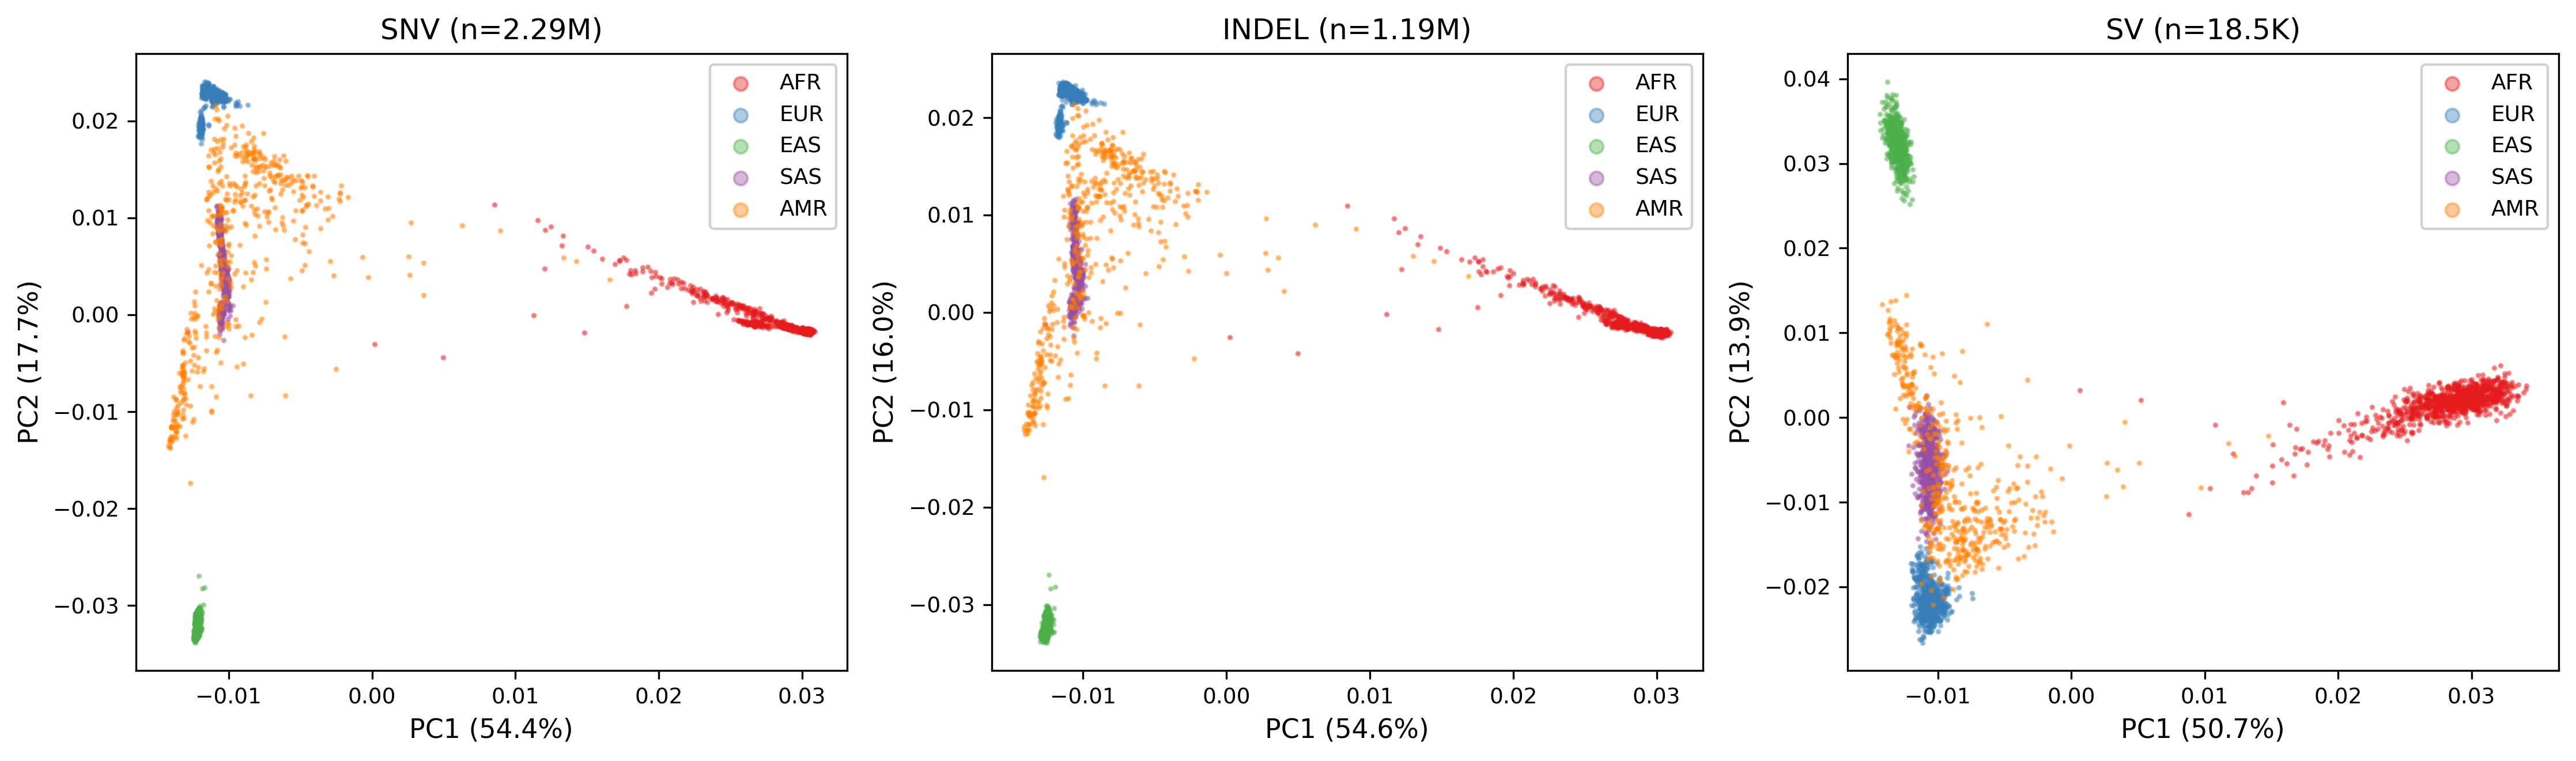
\includegraphics[width=\textwidth]{../figures/fig1_pca_comparison.png}
\caption{\textbf{Population structure across variant types.} Principal component analysis of 3,202 individuals from 26 populations using SNVs (left), INDELs (center), and SVs (right). All three variant types recover the five canonical continental super-population clusters (AFR, EUR, EAS, SAS, AMR). Percentage of variance explained by each PC is indicated on axes.}
\label{fig:overview}
\end{figure}

\begin{figure}[ht]
\centering
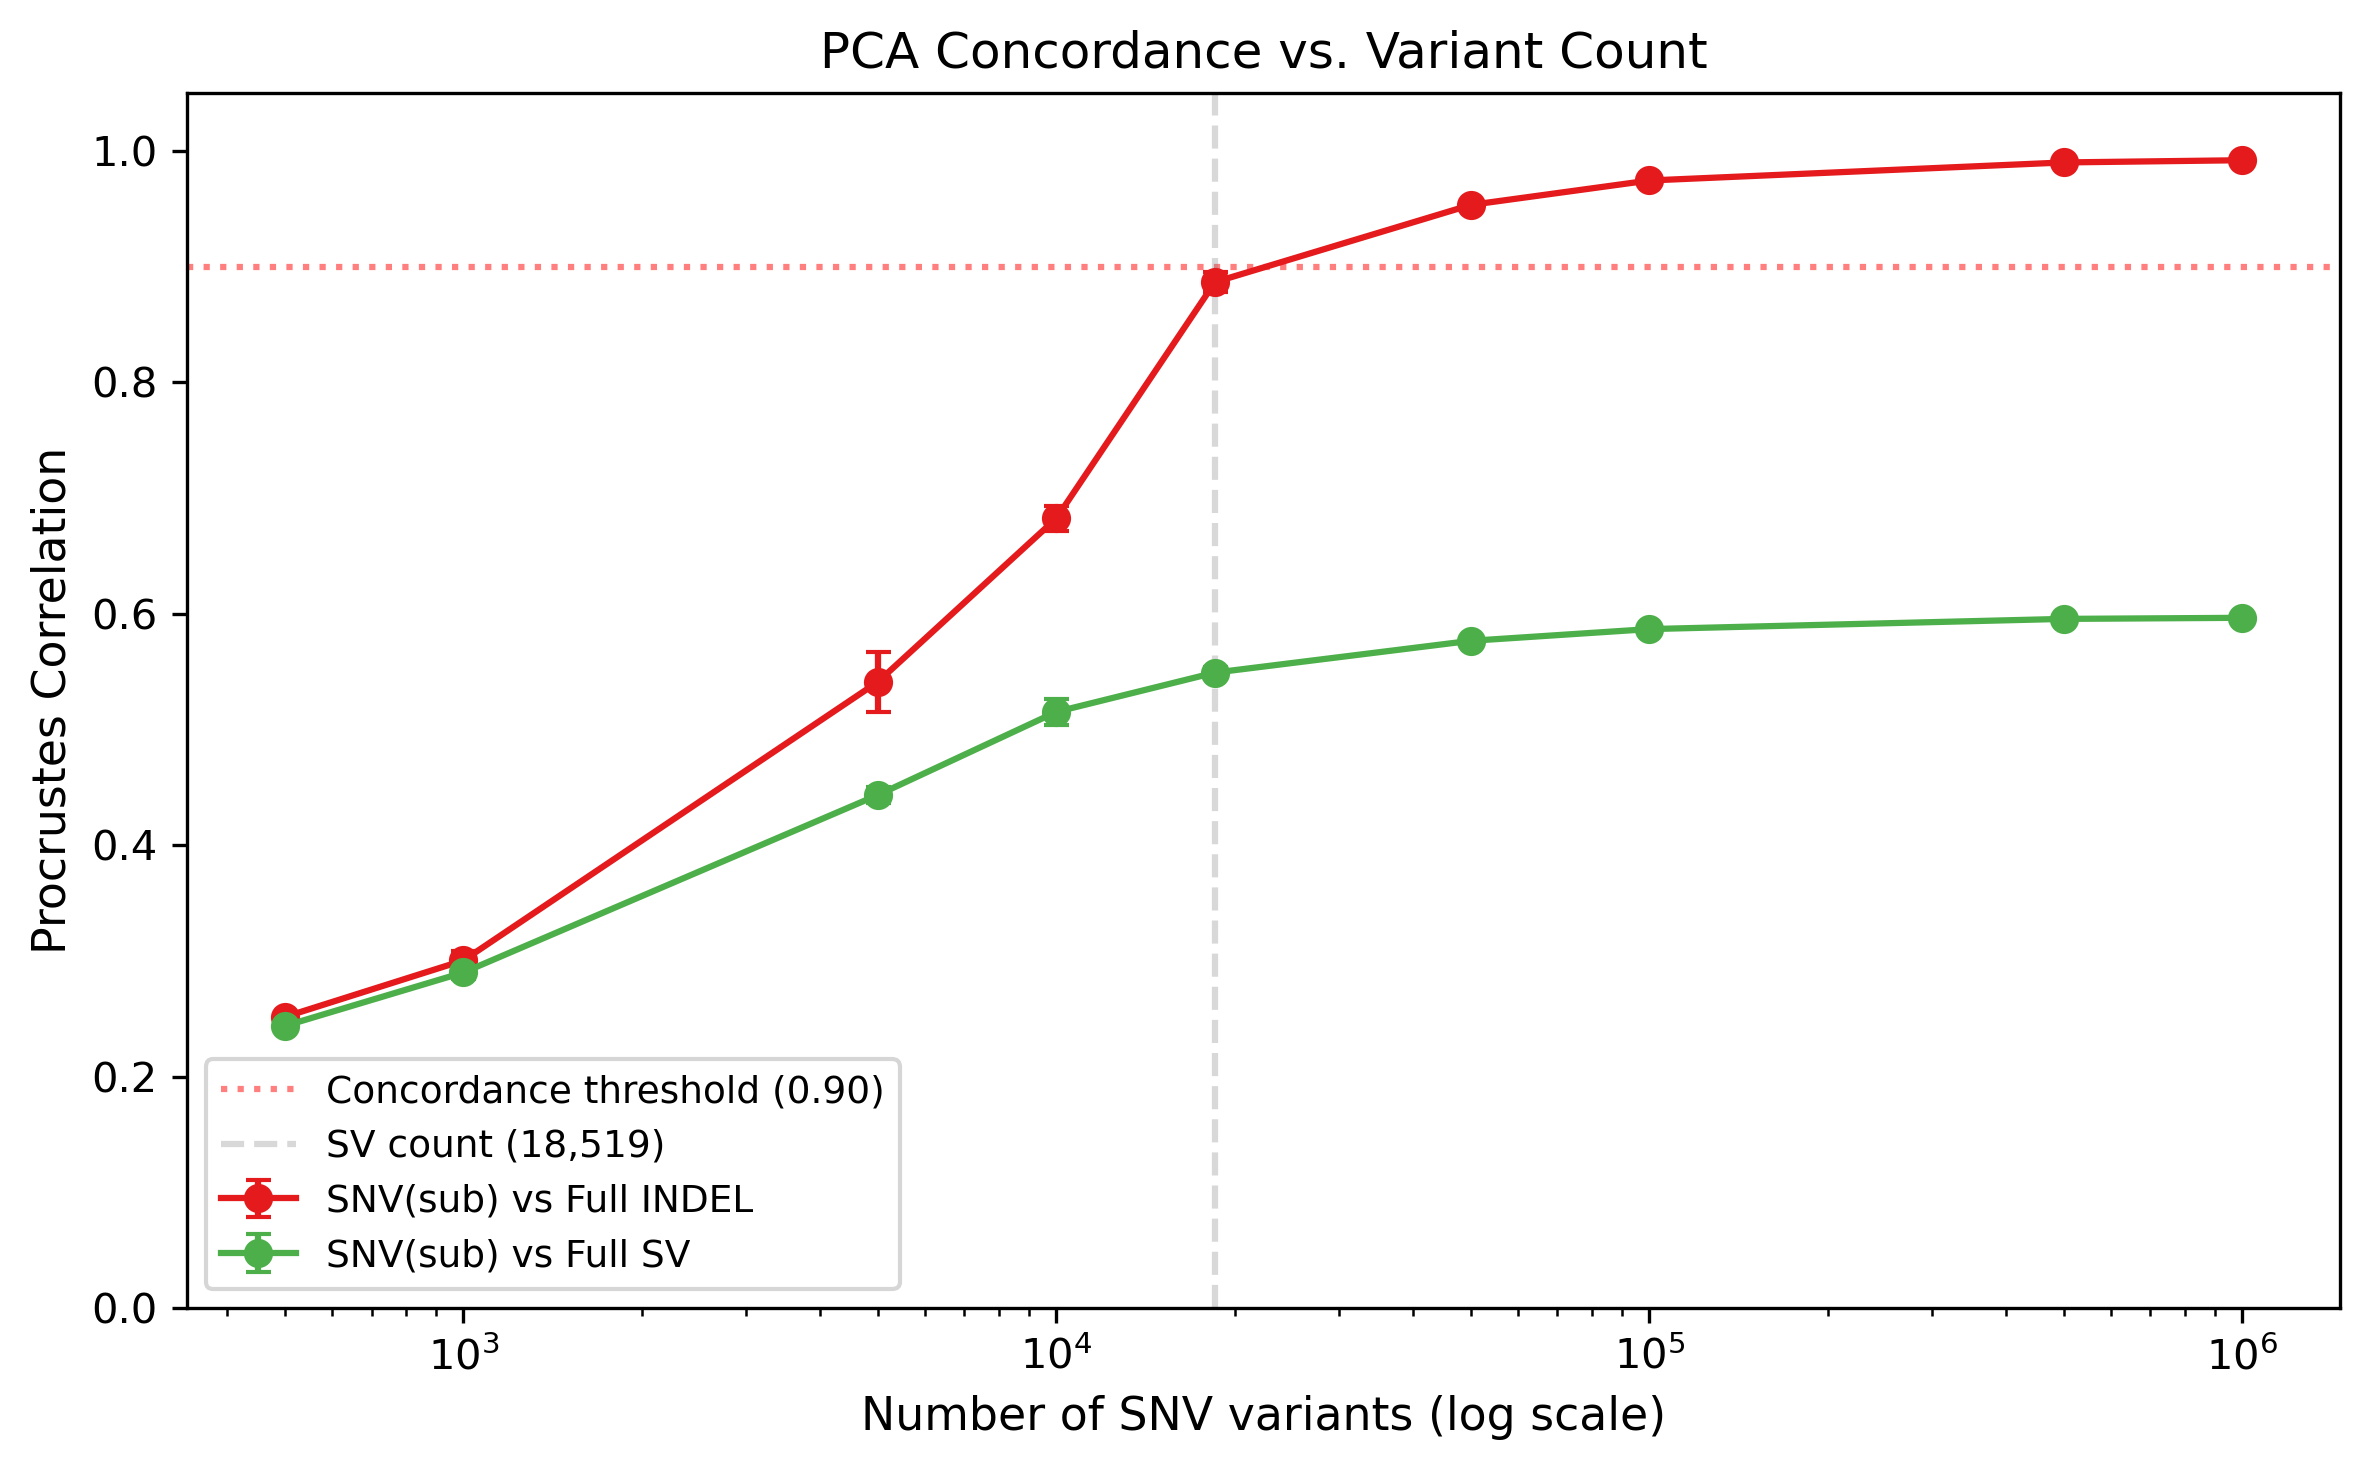
\includegraphics[width=0.85\textwidth]{../figures/fig_convergence_curve.png}
\caption{\textbf{Convergence analysis reveals irreducible SV discordance.} Procrustes correlation between subsampled SNV PCA and full INDEL (red) or full SV (green) PCA, as a function of the number of SNVs used. SNV-INDEL concordance rises monotonically and plateaus at $r \approx 0.99$ by $\sim$500,000 variants. SNV-SV concordance plateaus at $r \approx 0.60$ by $\sim$100,000 variants, establishing the discordance as biological signal rather than a power artifact. Error bars show standard deviation across three random seeds. Horizontal dashed line: concordance threshold (0.90). Vertical dashed line: SV count (18,519).}
\label{fig:convergence}
\end{figure}

\begin{figure}[ht]
\centering
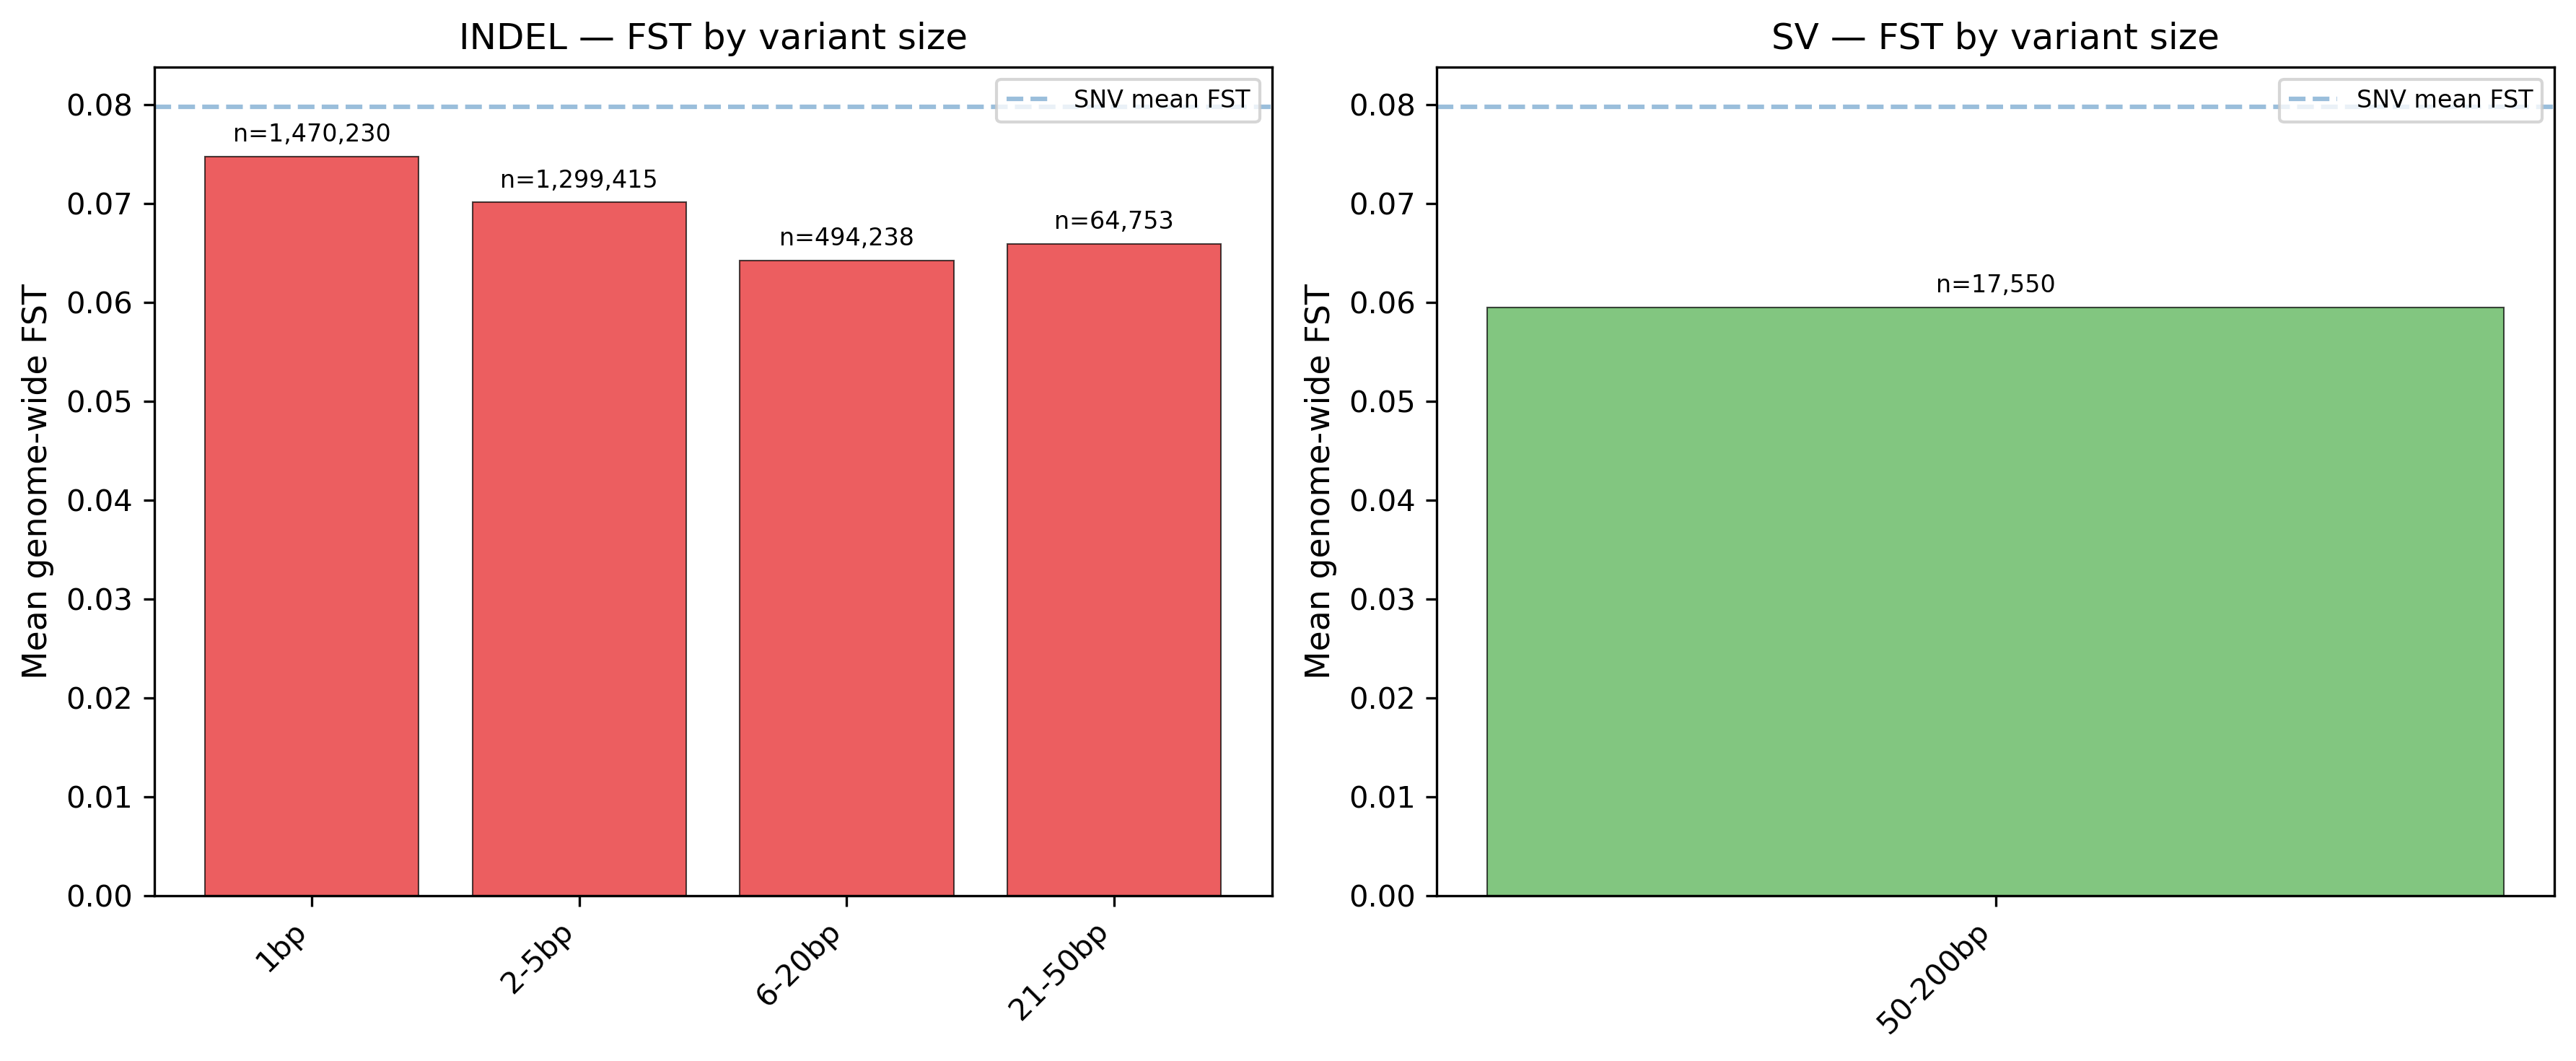
\includegraphics[width=\textwidth]{../figures/fig_size_stratified_fst.png}
\caption{\textbf{Size-dependent population differentiation gradient.} (A) Mean genome-wide $\fstmath$ across all 325 population pairs for INDELs stratified by size (left) and SVs (right). $\fstmath$ declines monotonically from 0.075 (1~bp INDELs) to 0.060 (50--200~bp SVs). Variant counts per bin shown above bars. Dashed blue line: SNV mean $\fstmath$ for reference. (B) SV subtype comparison showing 25\% lower $\fstmath$ for insertions (0.046) than deletions (0.062).}
\label{fig:size}
\end{figure}

\begin{figure}[ht]
\centering
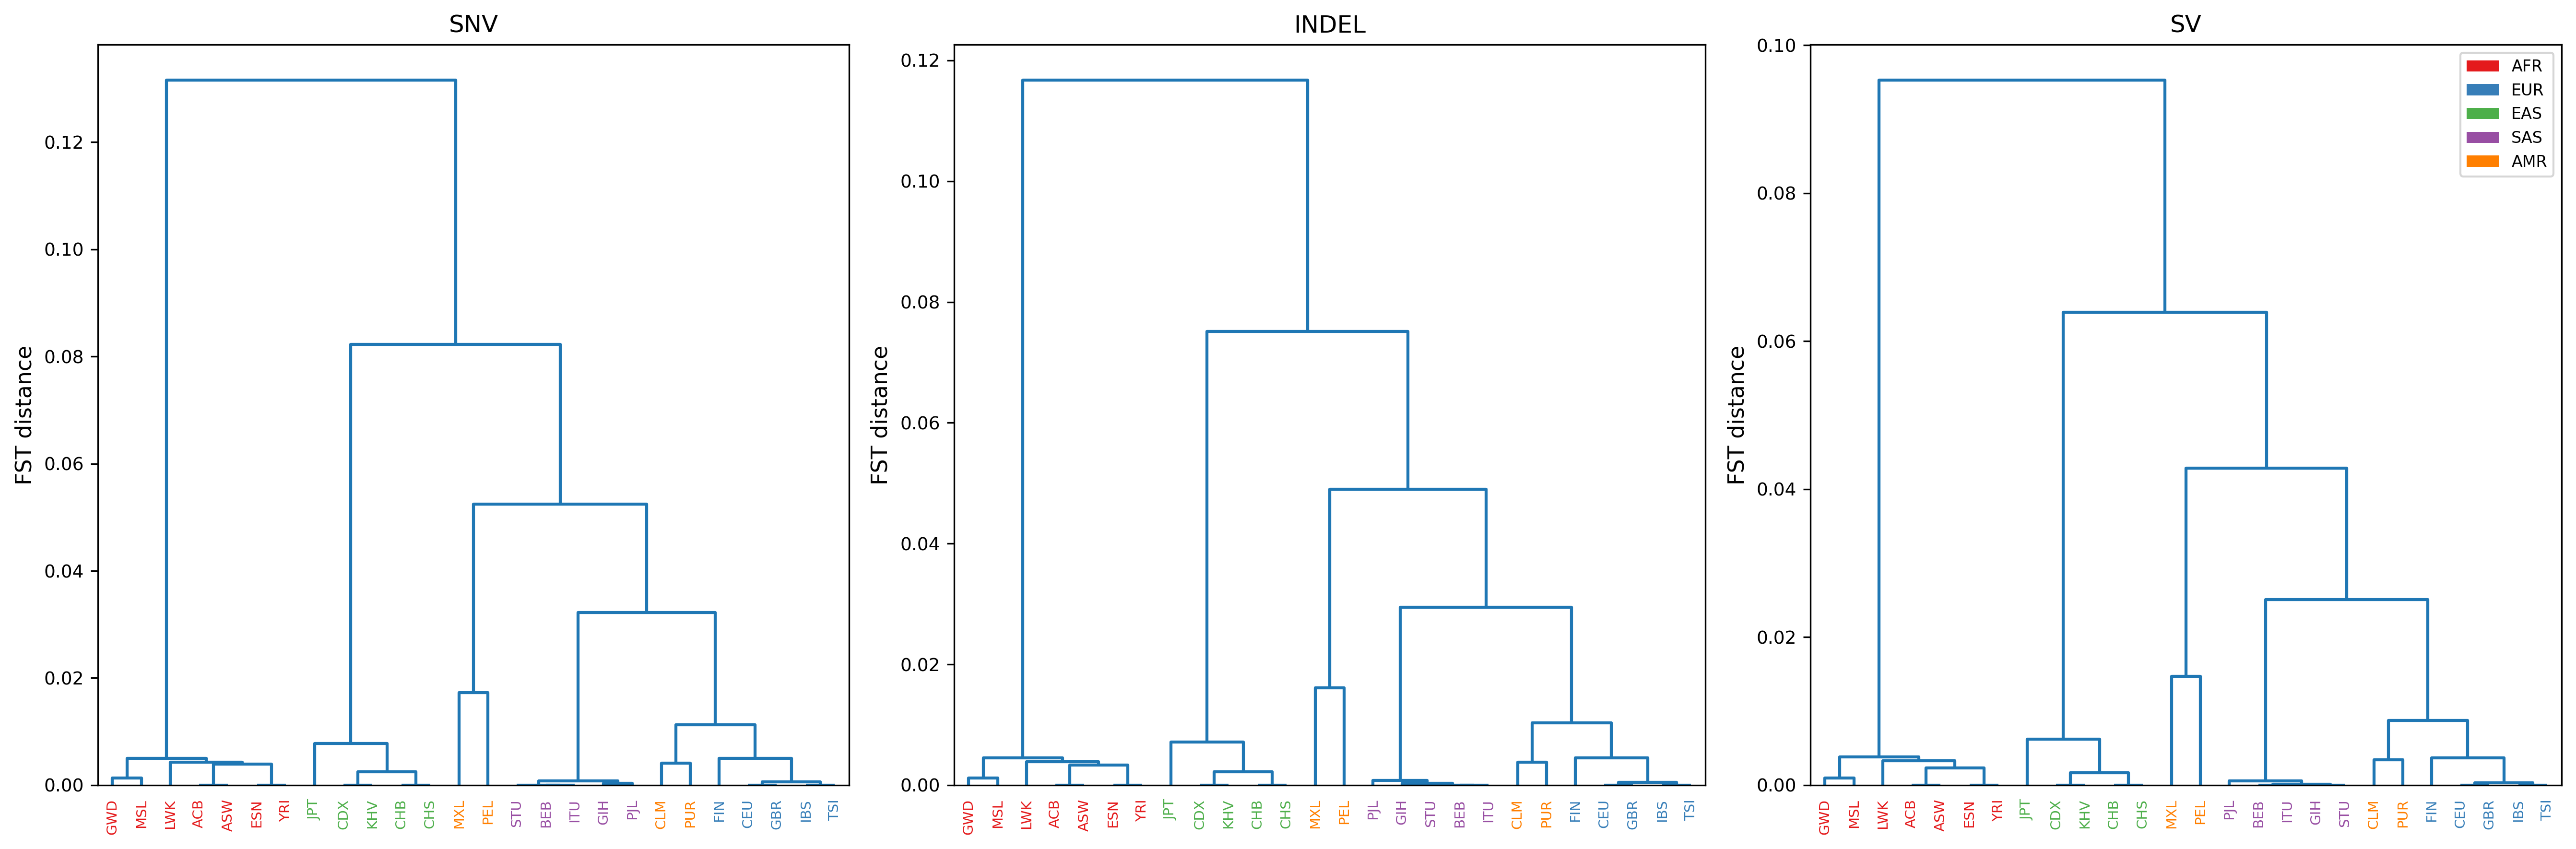
\includegraphics[width=0.9\textwidth]{../figures/fig7_population_trees.png}
\caption{\textbf{Population trees from $\fstmath$ distance matrices.} UPGMA dendrograms constructed from pairwise $\fstmath$ for SNVs, INDELs, and SVs. All three trees show concordant topology with the five super-populations forming monophyletic groups. Branch lengths differ systematically, with SVs showing compressed distances consistent with the $\fstmath$ attenuation gradient.}
\label{fig:trees}
\end{figure}

\begin{table}[ht]
\centering
\caption{\textbf{Cross-variant-type concordance summary.} Procrustes correlation, Mantel $r$, and $\fstmath$ correlation for each pair of variant types. Procrustes and Mantel values are based on the first 10 PCs. $\fstmath$ correlations are computed across 325 population pairs. All $p$-values $< 0.001$ (permutation-based for Procrustes and Mantel; asymptotic for Pearson/Spearman $\fstmath$ correlation).}
\label{tab:concordance}
\begin{tabular}{lccccc}
\toprule
Comparison & Procrustes $r$ & Mantel $r$ & $\fstmath$ Pearson $r$ & $\fstmath$ Spearman $\rho$ & $\fstmath$ slope \\
\midrule
SNV vs.\ INDEL & 0.993 & 0.998 & 0.9997 & 0.9995 & 0.886 \\
SNV vs.\ SV    & 0.598 & 0.781 & 0.9976 & 0.9974 & 0.723 \\
INDEL vs.\ SV  & 0.605 & 0.781 & 0.9989 & 0.9986 & 0.816 \\
\bottomrule
\end{tabular}
\end{table}

\begin{table}[ht]
\centering
\caption{\textbf{Size-stratified population differentiation.} Mean genome-wide $\fstmath$ computed across all 325 population pairs for each variant size category. The gradient from 1~bp INDELs to 50--200~bp SVs represents a 20\% reduction in population differentiation.}
\label{tab:sizefst}
\begin{tabular}{lrrc}
\toprule
Size category & $n$ variants & Mean $\fstmath$ & Type \\
\midrule
1 bp      & 1,470,230 & 0.0748 & INDEL \\
2--5 bp   & 1,299,415 & 0.0701 & INDEL \\
6--20 bp  & 494,238   & 0.0643 & INDEL \\
21--50 bp & 64,753    & 0.0659 & INDEL \\
50--200 bp & 17,550   & 0.0595 & SV \\
\midrule
\multicolumn{4}{l}{\textit{SV subtypes}} \\
DEL       & 14,091    & 0.0615 & SV \\
INS       & 4,428     & 0.0462 & SV \\
\bottomrule
\end{tabular}
\end{table}
